\section{对偶单纯形法}
\label{sec:simplex-dual}

工厂解完问题后，资源情况变了：原料增加到$13$，工时骤减到$2$，设备增加到$4$。这就需要回答：手里的最优基还能怎样利用，而不必从头求解？

\paragraph{基的两种可行性}
约化成本只依赖$\bm{c}$和基，与$\bm{b}$无关。所以右端变化后，原来的最优基$(1,5,2)$依然满足$\bm{s}\geq\bm{0}$，也就是对偶可行。受影响的是基变量。用式~\eqref{eq:simplex-final-inverse}的逆矩阵计算，新的基变量是
\[
 \bm{x}_B=\bm{A}_B^{-1}\begin{bmatrix}13\\2\\4\end{bmatrix}=\begin{bmatrix}-3\\-4\\8\end{bmatrix}.
\]
基失去了原始可行性，而对偶可行性完好。这正好与上一节相反：原始单纯形法保持$\bm{x}_B\geq\bm{0}$，逐步争取$\bm{s}\geq\bm{0}$；现在我们手里是$\bm{s}\geq\bm{0}$，需要逐步争取$\bm{x}_B\geq\bm{0}$。\term{对偶单纯形法}（dual simplex method）做的就是这件事。

\paragraph{主要思想}
选一个$\bar{x}_{B(r)}<0$的位置，让这个基变量出基。写出第$r$行，由式~\eqref{eq:simplex-basic-form}和式~\eqref{eq:simplex-row-coefficients}，每个满足等式的点都有
\begin{equation}
 x_{B(r)}+\sum_{j\in N}\bar{a}_{r,j}x_j=\bar{x}_{B(r)}<0.
 \label{eq:simplex-dual-row}
\end{equation}
要把$x_{B(r)}$抬到零，必须让某个$\bar{a}_{r,j}<0$的非基变量变大。候选可能有好几个，选哪一个由对偶可行性决定。

换到对偶的角度看。沿方向$\bm{\rho}$改变对偶变量，令$\bm{y}(\tau)=\bm{y}-\tau\bm{\rho}$，$\tau\geq0$。第一，对偶目标增大，这是我们想要的：
\[
 \bm{b}^\top\bm{y}(\tau)=\bm{b}^\top\bm{y}-\tau\,\bar{x}_{B(r)},
\]
这里用到了$\bm{\rho}^\top\bm{b}=\bar{x}_{B(r)}$。第二，约化成本线性变化：
\begin{equation}
 s_j(\tau)=c_j-\bm{a}_j^\top\bm{y}+\tau\,\bm{a}_j^\top\bm{\rho}=s_j+\tau\,\bar{a}_{r,j}.
 \label{eq:simplex-dual-reduced-cost}
\end{equation}
其他基变量的$\bar{a}_{r,j}=0$，它们的约化成本保持为零；第$r$个基变量的$\bar{a}_{r,j}=1$，约化成本变为$\tau\geq0$。非基变量中$\bar{a}_{r,j}\geq0$的不会变差，$\bar{a}_{r,j}<0$的会下降，下降到零时就必须停止。这就是对偶的比值检验：
\begin{equation}
 \tau^\star=\min_{j\in N:\,\bar{a}_{r,j}<0}\frac{s_j}{-\bar{a}_{r,j}}.
 \label{eq:simplex-dual-ratio}
\end{equation}
取到最小值的$q$入基，它的约化成本恰好变成零，所有约化成本仍然非负。

对比原始比值检验：原始检验防止基变量变负，选最先碰零的基变量出基；对偶检验防止约化成本变负，选最先碰零的非基变量入基。两者结构完全对称。表~\ref{tab:simplex-primal-dual-comparison}列出这种对称。

\begin{BookInlineTable}
 \centering
 \begin{tabular}{lll}
  \toprule
  & 原始单纯形法 & 对偶单纯形法\\
  \midrule
  保持 & $\bm{x}_B\geq\bm{0}$ & $\bm{s}\geq\bm{0}$\\
  争取 & $\bm{s}\geq\bm{0}$ & $\bm{x}_B\geq\bm{0}$\\
  先选 & $s_q<0$，入基 & $\bar{x}_{B(r)}<0$，出基\\
  比值检验选 & 出基位置 & 入基下标\\
  目标值 & 单调下降 & 单调上升\\
  否定结论 & 无界 & 不可行\\
  \bottomrule
 \end{tabular}
 \caption{原始单纯形法与对偶单纯形法的对照。}
 \label{tab:simplex-primal-dual-comparison}
\end{BookInlineTable}

式~\eqref{eq:simplex-dual-row}也解释了没有候选时的结论。若所有$\bar{a}_{r,j}\geq0$，式~\eqref{eq:simplex-dual-row}左端对任何$\bm{x}\geq\bm{0}$都非负，右端却是负数，所以无解。

\begin{theorem}[对偶单纯形法的不可行证书]
 \label{thm:simplex-dual-infeasible}
 设$\bar{x}_{B(r)}<0$，且所有$j\in N$都有$\bar{a}_{r,j}\geq0$，则$\bm{A}\bm{x}=\bm{b}$，$\bm{x}\geq\bm{0}$无解，$\bm{\rho}$满足
 \begin{equation}
  \bm{A}^\top\bm{\rho}\geq\bm{0},\qquad \bm{b}^\top\bm{\rho}=\bar{x}_{B(r)}<0.
  \label{eq:simplex-dual-certificate}
 \end{equation}
\end{theorem}

\begin{proof}
 基列的$\bm{\rho}^\top\bm{a}_j$是$0$或$1$，非基列的$\bm{\rho}^\top\bm{a}_j=\bar{a}_{r,j}\geq0$，所以$\bm{A}^\top\bm{\rho}\geq\bm{0}$；$\bm{b}^\top\bm{\rho}$是$\bm{A}_B^{-1}\bm{b}$的第$r$个分量。若有可行点$\bm{x}$，则
 \[
  0\leq\bm{x}^\top\bm{A}^\top\bm{\rho}=\bm{b}^\top\bm{\rho}<0,
 \]
 矛盾。
\end{proof}

\needspace{6\baselineskip}
\paragraph{变量}
沿用原始单纯形法的$B^{(t)},\bm{x}_B^{(t)},\bm{y}^{(t)},\bm{s}^{(t)},\bm{u}^{(t)}$，另增下面的量。
\begin{itemize}
 \item $r^{(t)}$：出基位置，$p^{(t)}=B^{(t)}(r^{(t)})$是出基下标。
 \item $\bm{\rho}^{(t)}\in\mathbb{R}^m$：$\bm{A}_B^{-\top}\bm{e}_r$；$\bar{a}_{r,j}^{(t)}$：第$r$行对第$j$列的系数。
 \item $\tau^{(t)}\geq0$：对偶步长；$q^{(t)}$：入基下标；$\alpha^{(t)}$：原始步长。
\end{itemize}

\paragraph{初始化}
需要一个对偶可行基。例中取原来的最优基，数据由式~\eqref{eq:simplex-resource-dual}和上面的计算得到：
\[
 B^{(0)}=(1,5,2),\qquad \bm{x}_B^{(0)}=(-3,-4,8)^\top,\qquad \bm{y}^{(0)}=(-2,-1,0)^\top.
\]
约化成本是$s_3=2$，$s_4=1$，对偶目标$\bm{b}^\top\bm{y}^{(0)}=-28$。这个$-28$比原问题的最优值低，它是新问题最优值的一个下界，算法要把它抬高。

\needspace{6\baselineskip}
\paragraph{每轮更新}
第$t$轮依次做下面几步。步骤后的“例中”是第$0$轮的数据。
\begin{enumerate}

 \item 判别。若$\bm{x}_B^{(t)}\geq\bm{0}$，停止，当前解最优。否则选负分量位置$r$出基，常取最负的。例中最负的是$x_5=-4$：
 \[
  r^{(0)}=2,\qquad p^{(0)}=5.
 \]

 \item 计算第$r$行。由式~\eqref{eq:simplex-row-coefficients}，例中取式~\eqref{eq:simplex-final-inverse}的第$2$行：
 \[
  \bm{\rho}^{(0)}=\Bigl(-\frac23,\frac13,1\Bigr)^\top,\qquad
  \bar{a}_{2,3}=-\frac23,\qquad \bar{a}_{2,4}=\frac13.
 \]

 \item 对偶比值检验。若所有$\bar{a}_{r,j}\geq0$，停止，按定理~\ref{thm:simplex-dual-infeasible}报告不可行。否则由式~\eqref{eq:simplex-dual-ratio}确定$\tau^{(t)}$和$q^{(t)}$。例中只有$x_3$是候选：
 \[
  \tau^{(0)}=\frac{2}{2/3}=3,\qquad q^{(0)}=3.
 \]

 \item 更新对偶量。沿$\bm{\rho}$移动，由式~\eqref{eq:simplex-dual-reduced-cost}更新约化成本：
 \begin{equation}
  \bm{y}^{(t+1)}=\bm{y}^{(t)}-\tau^{(t)}\bm{\rho}^{(t)},\qquad
  s_j^{(t+1)}=s_j^{(t)}+\tau^{(t)}\bar{a}_{r,j}^{(t)}.
  \label{eq:simplex-dual-update}
 \end{equation}
 例中
 \[
  \bm{y}^{(1)}=(0,-2,-3)^\top,\qquad s_4^{(1)}=1+3\cdot\frac13=2,\qquad s_5^{(1)}=3.
 \]

 \item 更新原始量。先求$\bm{u}^{(t)}=\bm{A}_B^{-1}\bm{a}_q$，取原始步长$\alpha^{(t)}=\bar{x}_{B(r)}/\bar{a}_{r,q}$，它是让第$r$个基变量恰好变成零的步长。其余基变量按式~\eqref{eq:simplex-primal-update}更新，第$r$个位置放$x_q=\alpha^{(t)}$。例中
 \[
  \bm{u}^{(0)}=\Bigl(-\frac13,-\frac23,\frac23\Bigr)^\top,\qquad
  \alpha^{(0)}=\frac{-4}{-2/3}=6.
 \]
 于是
 \[
  B^{(1)}=(1,3,2),\qquad \bm{x}_B^{(1)}=(-1,6,4)^\top,\qquad \bm{b}^\top\bm{y}^{(1)}=-16.
 \]
\end{enumerate}

例中第$1$轮只剩$x_1=-1$为负，所以$r=1$，$x_1$出基。第$1$行的系数和唯一的候选是
\[
 \bm{\rho}^{(1)}=\Bigl(0,\frac12,-\frac12\Bigr)^\top,\qquad
 \bar{a}_{1,4}=\frac12,\qquad \bar{a}_{1,5}=-\frac12,\qquad
 \tau^{(1)}=\frac{3}{1/2}=6.
\]
于是$x_5$入基，由式~\eqref{eq:simplex-dual-update}得到
\[
 \bm{y}^{(2)}=(0,-5,0)^\top,\qquad s_1^{(2)}=6,\qquad s_4^{(2)}=2+6\cdot\frac12=5.
\]
原始量的更新用
\[
 \bm{u}^{(1)}=\Bigl(-\frac12,-\frac32,1\Bigr)^\top,\qquad
 \alpha^{(1)}=\frac{-1}{-1/2}=2,
\]
更新后得到
\[
 B^{(2)}=(5,3,2),\qquad \bm{x}_B^{(2)}=(2,9,2)^\top,\qquad \bm{b}^\top\bm{y}^{(2)}=-10.
\]
第$2$轮$\bm{x}_B\geq\bm{0}$，算法停止。

\paragraph{最终得到}
新问题的最优解和最优值是
\[
 (x_1,x_2)=(0,2),\qquad p^\star=-10.
\]
工时只有$2$，全部给利润率更高的产品二最合算。对偶目标依次是$-28,-16,-10$，每一步增加$\tau\lvert\bar{x}_{B(r)}\rvert$，即$3\cdot4=12$和$6\cdot1=6$，它们一直是最优值的下界，到达时恰好等于最优值。这与第~\ref{sec:simplex-basis-exchange}节目标从上方下降的情形相反。

图~\ref{fig:simplex-dual-path}(a)显示了路径的特点：前两个点$(-3,8)$和$(-1,4)$都在可行域之外，它们是一系列“太便宜而不可能达到”的解，算法一步步向可行域靠拢，碰到可行域时恰好最优。

\begin{BookInlineFigure}
 \centering
 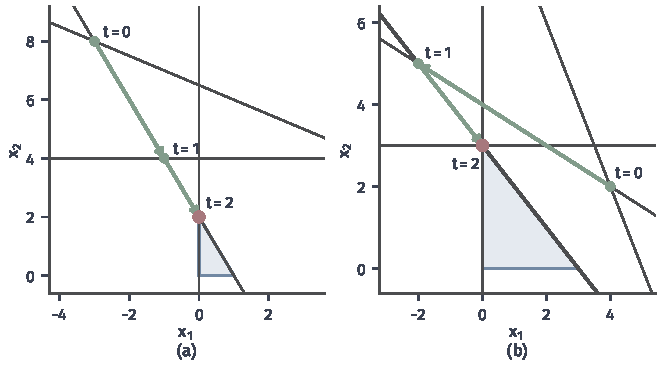
\includegraphics[width=112mm]{figures/05-optimization/01-linear-programming/matplotlib/simplex-dual-path/figure.pdf}
 \caption{对偶单纯形法在原始空间的路径（绿色），深灰线是约束边界，浅蓝是可行域，红点是最优解。(a)~右端变为$(13,2,4)$后，从不可行点$(-3,8)$经$(-1,4)$到$(0,2)$。(b)~新增约束$x_1+x_2\leq3$（粗线）后，从原最优点$(4,2)$经不可行点$(-2,5)$到$(0,3)$。}
 \label{fig:simplex-dual-path}
\end{BookInlineFigure}

\paragraph{新增约束与基的复用}
加入新约束是另一种常见的情形。给工厂加一条约束$x_1+x_2\leq3$，并引入松弛变量$x_6$。把$x_6$放入基，原最优基扩展成$(1,5,2,6)$。新基对偶可行，因为新列只增加一个取零的约化成本；只有$x_6$可能违反非负，这里$x_6=3-6=-3$。

第$0$轮$x_6$出基，第$4$行的系数和两个候选比值是
\[
 \bar{a}_{4,3}=-\frac13,\qquad \bar{a}_{4,4}=-\frac13,\qquad
 \frac{2}{1/3}=6,\qquad \frac{1}{1/3}=3.
\]
图~\ref{fig:simplex-dual-ratio}把这两个比值画成约化成本随$\tau$下降的直线，$s_4$先碰到零，所以$x_4$入基。再经一轮换基，$\bm{x}_B$全部非负，得到$(x_1,x_2)=(0,3)$，利润$15$。

\begin{BookInlineFigure}
 \centering
 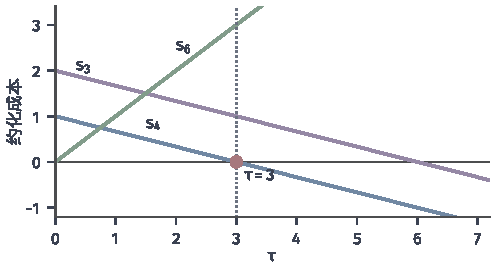
\includegraphics[width=84mm]{figures/05-optimization/01-linear-programming/matplotlib/simplex-dual-ratio/figure.pdf}
 \caption{新增约束后第$0$轮的对偶比值检验。三条直线是约化成本随对偶步长$\tau$的变化：$s_3=2-\tau/3$，$s_4=1-\tau/3$，$s_6=\tau$。红点是最先降到零的位置$\tau=3$，它决定入基变量$x_4$；$s_6$对应出基的$x_6$，只增不减。}
 \label{fig:simplex-dual-ratio}
\end{BookInlineFigure}

如果新增的约束与资源不相容，比如$x_1+x_2\geq7$，化为$-x_1-x_2+x_6=-7$后，第一轮$x_6=-1$，第$4$行是
\[
 x_6+\frac13x_3+\frac13x_4=-1.
\]
系数全部非负而右端为负，这正是定理~\ref{thm:simplex-dual-infeasible}的情形，算法一步报告不可行。这和第~\ref{sec:simplex-two-phase}节第一阶段得到的结论相同，证书都是原料和工时约束的组合。

这种利用已有基的做法称为\term{热启动}（warm start）。它是整数规划算法的基本工序：分支限界在线性松弛的解上增加一个变量界，割平面增加一条被当前解违反的不等式，两者都只在原问题上添一点约束，原来的最优基仍然对偶可行。对偶单纯形法往往只需少量换基就能恢复可行，比从头求解省得多。热启动的效果依赖新约束对解的改变有多大，并没有通用的步数保证。
